\begin{pastexam}[label={px:nsysu-107-osds-01}]{中山資工所甲組 107 學年度 第 5 題}
（問答）

\textbf{[Basic Data Structures: 15\%]}
\begin{enumerate}[label=(\arabic*)]
\item Consider a binary tree. Suppose that its DFS result is ``c, b, e, f, d, h, i, g, k, a, j''
while BFS result is ``c, b, g, e, d, k, j, f, h, i, a''. Please draw the tree. (3\%)
\item Given the postfix of an equation ``2 4 + 6 $\times$ 9 8 $-$ 3 5 + $\times$ $-$'', please
compute its result. List your calculation. (3\%)
\item What is a binary search tree? Explain its property. (2\%)
\item Except that every node is either red or black, how can you make a binary search tree become
a red-black tree? (4\%)
\item Show that the worst-case complexity of quicksort is O(n$^2$). (3\%)
\end{enumerate}
\end{pastexam}

\begin{pastsoln}
五個小題分屬不同章：(1) 樹的重建（資結書第~7.4~節）、(2) 後序式求值（第~6.3~節）、(3) 二元搜尋樹
（第~9~章）、(4) 紅黑樹（第~10.3~節）、(5) 快速排序（第~14.5~節）。

\textbf{(1)} 題目沒說 DFS 是哪一種。 二元樹的 DFS 一般指從根出發、先左後右的深度優先走訪，也就是
前序；BFS 是由上而下、每層由左到右的層序。 下面照這個解讀。

前序 \texttt{c b e f d h i g k a j}，層序 \texttt{c b g e d k j f h i a}。
\begin{itemize}
\item 根是 \texttt{c}（兩個序列的第一個）。 前序緊接著是 \texttt{b}，所以 \texttt{b} 是
\texttt{c} 的第一個子節點。
\item 層序第三個是 \texttt{g}。 如果 \texttt{c} 只有 \texttt{b} 一個子節點，層序接在 \texttt{b}
後面的就是 \texttt{b} 的子節點，而前序裡 \texttt{b} 的第一個子節點是 \texttt{e}，層序應該先出現
\texttt{e}，矛盾。 所以 \texttt{g} 是 \texttt{c} 的右子節點，\texttt{b} 是左子節點。 前序在
\texttt{g} 處切開：左子樹的前序是 \texttt{b e f d h i}，右子樹是 \texttt{g k a j}。
\item 第 $2$ 層（深度 $2$）在層序裡是 \texttt{e d k j}。 \texttt{b} 子樹裡是 \texttt{e}、\texttt{d}，
前序 \texttt{b e f d h i} 裡 \texttt{e} 在 \texttt{d} 前面，所以 \texttt{e} 左、\texttt{d} 右；
\texttt{e} 的子樹是 \texttt{e f}，\texttt{d} 的子樹是 \texttt{d h i}。 同理 \texttt{g} 的左右子節點
是 \texttt{k}、\texttt{j}，\texttt{k} 的子樹是 \texttt{k a}。
\item 第 $3$ 層是 \texttt{f h i a}：\texttt{f} 是 \texttt{e} 唯一的子節點；\texttt{h}、\texttt{i}
是 \texttt{d} 的左、右子節點；\texttt{a} 是 \texttt{k} 唯一的子節點。
\end{itemize}

\begin{center}
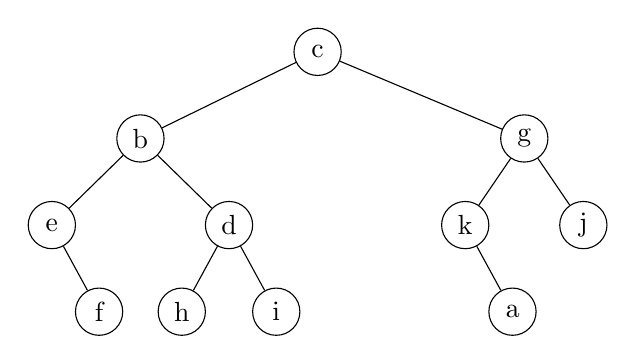
\begin{tikzpicture}[x=0.75cm,y=1.1cm,v/.style={circle,draw,inner sep=0pt,minimum size=6mm}]
\node[v] (c) at (6,0) {c};
\node[v] (b) at (3,-1) {b}; \node[v] (g) at (9.5,-1) {g};
\node[v] (e) at (1.5,-2) {e}; \node[v] (d) at (4.5,-2) {d};
\node[v] (k) at (8.5,-2) {k}; \node[v] (j) at (10.5,-2) {j};
\node[v] (f) at (2.3,-3) {f}; \node[v] (h) at (3.7,-3) {h}; \node[v] (i) at (5.3,-3) {i};
\node[v] (a) at (9.3,-3) {a};
\draw (c)--(b) (c)--(g) (b)--(e) (b)--(d) (g)--(k) (g)--(j) (e)--(f) (d)--(h) (d)--(i) (k)--(a);
\end{tikzpicture}
\end{center}
上圖把 \texttt{f}、\texttt{a} 畫成右子節點。 \textbf{答案不唯一}：\texttt{e} 和 \texttt{k} 都只有一個
子節點，前序和層序都看不出它是左還是右（只有一個子節點時，兩種放法的前序、層序完全相同）。 所以
\texttt{f} 可以是 \texttt{e} 的左或右子節點，\texttt{a} 可以是 \texttt{k} 的左或右子節點，一共
$2 \times 2 = 4$ 棵樹都符合，其他部分都是唯一的。 這和資結書定理~7.5 是同一個現象：給前序和後序時，符合的樹有
$2^m$ 棵，$m$ 是只有一個子節點的節點數；這裡 $m = 2$。 缺了中序，就分不出單一子節點的左右。 作答時畫一棵並註明
這一點即可。

\textbf{(2)} 答案是 $28$。 由左往右讀，數字推入堆疊；讀到運算子就彈出兩個數，先彈出的是右運算元
（資結書虛擬碼~6.7）：
\begin{center}
\begin{tabular}{cll}
\toprule
讀到 & 計算 & 堆疊（底 $\to$ 頂） \\
\midrule
2, 4 & & $2, 4$ \\
$+$ & $2 + 4 = 6$ & $6$ \\
6 & & $6, 6$ \\
$\times$ & $6 \times 6 = 36$ & $36$ \\
9, 8 & & $36, 9, 8$ \\
$-$ & $9 - 8 = 1$ & $36, 1$ \\
3, 5 & & $36, 1, 3, 5$ \\
$+$ & $3 + 5 = 8$ & $36, 1, 8$ \\
$\times$ & $1 \times 8 = 8$ & $36, 8$ \\
$-$ & $36 - 8 = 28$ & $28$ \\
\bottomrule
\end{tabular}
\end{center}
對應的中序式是 $(2 + 4) \times 6 - (9 - 8) \times (3 + 5) = 36 - 8 = 28$。

\textbf{(3)} 二元搜尋樹（binary search tree）是一棵二元樹，每個節點存一個鍵，而且對每個節點 $x$：
$x$ 左子樹裡\textbf{每一個}鍵都 $< x.\mathit{key}$，右子樹裡每一個鍵都 $> x.\mathit{key}$
（資結書定義~9.1；允許重複鍵時，把其中一邊改成 $\le$ 或 $\ge$）。 條件是對整棵子樹，不是只比父子。 這個性質的結果：
\begin{itemize}
\item 中序走訪會由小到大輸出所有的鍵（資結書定理~9.1）；
\item 搜尋、插入、刪除、找最小最大、前驅後繼，都只要沿著一條從根往下的路徑走，時間是 $O(h)$，
$h$ 是樹高；樹平衡時 $h = O(\lg n)$，最壞（例如依序插入排好的資料）退化成 $h = n$。
\end{itemize}

\textbf{(4)} 除了「每個節點是紅或黑」，還要滿足下面四條（資結書定義~10.2）：
\begin{enumerate}[label=(\roman*)]
\item 根是黑色。
\item 每個 NIL（外部節點、空的子樹）都是黑色。
\item 紅色節點的兩個子節點都是黑色，也就是不會有兩個紅色節點相連。
\item 對每個節點 $x$，從 $x$ 往下走到任何一個 NIL 的每條路徑，經過的黑色節點個數都一樣（叫 $x$ 的
黑高）。
\end{enumerate}
這四條合起來保證最長的根到 NIL 路徑不超過最短的兩倍，$n$ 個內部節點的紅黑樹高度
$\le 2\lg(n+1)$（資結書定理~10.4）。

\textbf{(5)} 令 $T(n)$ 是快速排序排 $n$ 個數的最壞時間。 分割 $n$ 個數要 $\Theta(n)$（基準和其他
$n - 1$ 個各比一次），設不超過 $cn$。 分割後基準左邊 $q$ 個、右邊 $n - 1 - q$ 個，$0 \le q \le n - 1$，
最壞情況要對所有可能的 $q$ 取最大：
\[
T(n) \le \max_{0 \le q \le n-1} \bigl(T(q) + T(n - 1 - q)\bigr) + cn .
\]
用代換法證明 $T(n) \le dn^2$（$d \ge c$，基底 $T(0)$、$T(1)$ 取 $d$ 夠大即可）。 歸納假設對比
$n$ 小的都成立，則
\[
T(n) \le d \max_{0 \le q \le n-1} \bigl(q^2 + (n-1-q)^2\bigr) + cn .
\]
$q^2 + (n-1-q)^2$ 是 $q$ 的開口向上的二次函數，最大值在端點 $q = 0$ 或 $q = n - 1$，等於 $(n-1)^2$。
所以
\[
T(n) \le d(n-1)^2 + cn = dn^2 - d(2n - 1) + cn \le dn^2,
\]
最後一步因為 $d(2n - 1) \ge dn \ge cn$（$n \ge 1$、$d \ge c$）。 得 $T(n) = O(n^2)$。

這個上界會達到：每次都切成 $0$ 和 $n - 1$（例如 Lomuto 分割取最後一個數當基準、輸入已經排好），比較
次數是 $(n-1) + (n-2) + \cdots + 1 = n(n-1)/2$，所以最壞情況其實是 $\Theta(n^2)$。
\end{pastsoln}
